\chapter{Existující aplikace}\label{chap:ExistingApps}

Existuje několik aplikací, které řeší problém simulace zásobníkových automatů. Tato kapitola se bude některým z nich věnovat.

% BIB: https://github.com/davidbuzatto/YAAS
\section{YAAS --- Yet Another Automata Simulator}

YAAS --- Yet Another Automata Simulator, v češtině přeloženo jako Ještě Další Simulátor Automatů, je aplikace vytvořená profesorem Davidem Buzattem z Federálního institutu pro vzdělání, vědu a technologie v São Paulu. Tato aplikace obsahuje nejen možnost tvorby zásobníkových automatů, ale i konečných automatů a turingových strojů. Zásobníkové automaty se v aplikaci tvoří graficky --- uživatel se přidá stavy a pak mezi nimi může vytvářet přechody. Aplikace si z těchto informací sama vytvoří příslušnou vstupní a zásobníkovou abecedu. Při spuštění simulace se pak uživateli zobrazí posloupnost přechodů a zároveň v grafickém zobrazení obarvuj konkrétní stav, ve kterém se zrovna zásobníkový automat nachází, obrázek~\ref{fig:YAAS}

\begin{figure}[h]
    \centering
    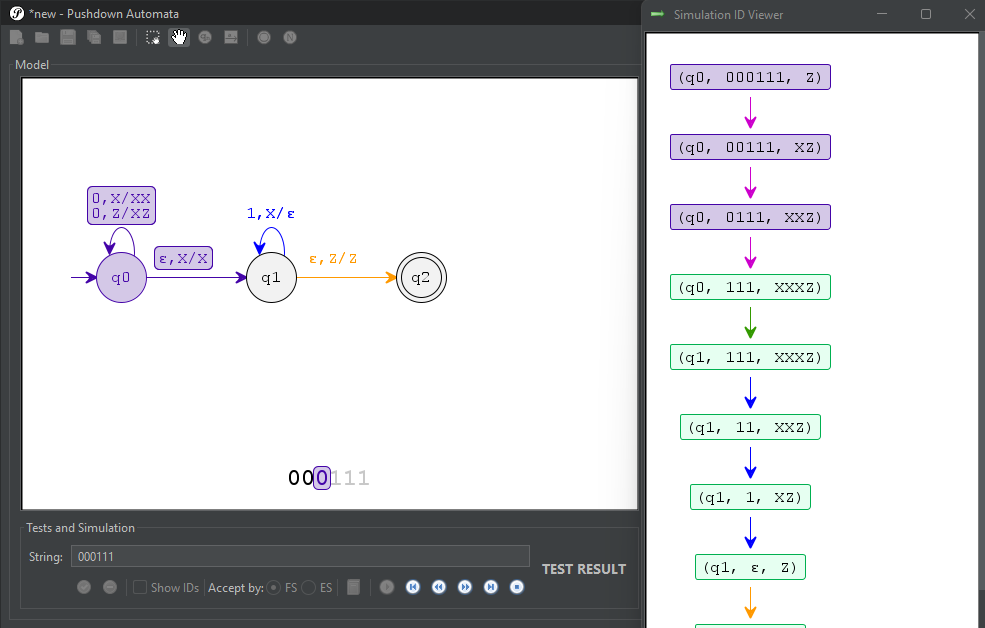
\includegraphics[width=\textwidth]{Figures/PrntScrn_YAAS.png}
    \caption{YAAS v průbehu simulace.}\label{fig:YAAS}
\end{figure}

% BIB: https://github.com/DauteRR/PushdownAutomaton
\section{DauteRR --- Pushdown Automaton}

Pushdown automaton od Dauta Rodríguez Rodrígueze je konzolová aplikace napsaná v jazyce Java. Tato aplikace na vstup bere soubor s definicí zásobníkového automatu. Vstupy jsou zadány buď v druhém vstupním souboru nebo jsou čteny z příkazového řádku. Program dále umožňuje zapnout tzv.~trace mód, který ve výpisu ukazuje jednotlivé kroky a pomocí > označuje, který symbol je zrovna čtený.

\section{Bakalářsá práce}

%TODO: nefunguje DSPACE
Ahhhhhhhhhhhhhhhhhhh

\endinput